% Hauptdatei des Projektes. Von hier aus werden die anderen Seiten eingebunden
%!TEX root = ../konzeptpapier.tex

\documentclass[12pt,a4paper]{article}
\usepackage[utf8]{inputenc}
\usepackage[ngerman]{babel}
\usepackage[T1]{fontenc}
\usepackage{amsmath}
\usepackage{amsfonts}
\usepackage{amssymb}
\usepackage{xspace}
\usepackage{graphicx}
\usepackage{color}

%%%%%%%%%%%%%%%%%%%%%%%%%%%%%%%%%%%%%%%%%%%%%%%%%%%%%%%%%%%%%%%%%%%%%%%%%%%%%%%%%%%%%%%%%%
% In diesem Abschnitt gibst du deine persönlichen Daten sowie den Kontext deiner Arbeit an
% das \xspace am Ende der Einträge muss vorhanden bleiben. Es regelt das Whitespace-
% handling
%%%%%%%%%%%%%%%%%%%%%%%%%%%%%%%%%%%%%%%%%%%%%%%%%%%%%%%%%%%%%%%%%%%%%%%%%%%%%%%%%%%%%%%%%%
% persönliche Daten
\newcommand{\vorname}{Hier dein Vorname\xspace}
\newcommand{\nachname}{Hier dein Nachname\xspace}
\newcommand{\emailadresse}{Hier deine Mailadresse\xspace}
\newcommand{\matrikelnummer}{Hier deine Matrikelnummer\xspace}


% Arbeitsspezifische Daten
\newcommand{\titel}{Konzeptpapier Multimediaprodukt\xspace}
\newcommand{\untertitel}{Hier der Untertitel der Arbeit\xspace}
\newcommand{\modulname}{Hier der Modulname\xspace}
\newcommand{\pruefer}{Hier der vollständige Name des Prüfers\xspace}
\newcommand{\semester}{Das Semester\xspace}
\newcommand{\ortderarbeit}{Hier der Ort für die Erklärung der Selsbtständigkeit\xspace}
%%%%%%%%%%%%%%%%%%%%%%%%%%%%%%%%%%%%%%%%%%%%%%%%%%%%%%%%%%%%%%%%%%%%%%%%%%%%%%%%%%%%%%%%%%

%Hurenkinder uns Schusterjungen
\clubpenalty10000
\widowpenalty10000
\displaywidowpenalty=10000

\usepackage{hyperxmp} % XMP-Daten fuer die PDF-Datei
%Gimmmick: Linked Kapitel und Inhaltsverzeichnis, sowie Referenzen
\usepackage[pdftex, pdfa]{hyperref}
\hypersetup{
    colorlinks,
    citecolor=black,
    filecolor=black,
    linkcolor=black,
    urlcolor=black,
    pdftitle = {\titel},
    pdfauthor = {\vorname \nachname},
    pdfsubject = {\untertitel},
    pdfkeywords = {\titel \untertitel \matrikelnummer},
    pdflang = de,
    bookmarks = true,
    pdfdisplaydoctitle = true,
    colorlinks = true,
    plainpages = false,
    %allcolors = black,
    hypertexnames = false,
    pdfpagelabels = true,
    hyperindex = true,
    unicode = true,
    pdfcaptionwriter = {\textsl{\vorname \nachname}},
    pdfcontactaddress = {Eine Straße. 9},
    pdfcontactcity = {EinOrt},
    pdfcontactpostcode = {EinePostleitzahl},
    pdfcontactcountry = {Deutschland},
    pdfcontactregion = {EinBundesland},
    pdfcontactemail = {\emailadresse},
    pdfcontactphone = {EineTelefonnummer},
    pdfcontacturl = {http://www.hs-fulda.de},
    pdfmetalang = {de},
}

\usepackage{prettyref}
\usepackage{titleref}

%Schriftart
\usepackage{lmodern}
\usepackage{mathptmx}
\usepackage[scaled=.90]{helvet}

\usepackage{courier}
%Inhaltsverzeichnis
\usepackage[tocgraduated]{tocstyle}
\usetocstyle{allwithdot}
\setcounter{tocdepth}{3}

% Formatierungshilfen: http://wwws.htwk-leipzig.de/~myagovki/latex/formatierungshilfen/

\usepackage[ddmmyyyy]{datetime}
\renewcommand{\dateseparator}{.}

% Für Kopf und Fußzeile: https://esc-now.de/_/latex-individuelle-kopf--und-fusszeilen/?lang=en
\usepackage[
  headsepline, plainheadsepline,
  footsepline, plainfootsepline
]{scrlayer-scrpage}
\pagestyle{scrheadings}
\clearscrheadfoot

\ihead*{\titel}
\ohead*{\vorname\:\nachname}
\ifoot*{\modulname}
\ofoot*{\pagemark}
\AtEndDocument{\ofoot{}}

% anderthalbfacher Zeilenabstand
\usepackage[onehalfspacing]{setspace}

%Geometry der Seite festlegen
\usepackage{geometry}
\geometry{
  left=2.5cm,
  right=5cm,
  top=2.5cm,
  bottom=2cm,
  headheight=33pt
}

%Für Gestaltung des Layouts
\usepackage{blindtext}


%Bilbliothek und Literatur einbinden

\usepackage[style=authoryear-ibid,natbib=true,backend=biber,sorting=nty,hyperref=true]{biblatex}
\usepackage[babel,german=guillemets]{csquotes}
\addbibresource{bib/literatur.bib}


\newcommand{\zb}{z.\,B.\xspace}







%https://www.dante.de/events/dante2015/Programm/vortraege/vortrage-partosch2.pdf


\immediate\pdfobj stream attr{/N 3} file{res/AdobeRGB1998.icc}
\pdfcatalog{%
/OutputIntents [ <<
/Type /OutputIntent
/S/GTS_PDFA1
/DestOutputProfile \the\pdflastobj\space 0 R
/OutputConditionIdentifier (Adobe RGB 1998)
/Info(Adobe RGB 1998)
>> ]
}

\input{glyphtounicode.tex}
\input{glyphtounicode-cmr.tex}
\pdfgentounicode=1
\pdfobjcompresslevel=0
\pdfinclusioncopyfonts=1


\begin{document}

%\pagenumbering{Alph}
%!TEX root = ../konzeptpapier.tex
\begin{titlepage}
\newgeometry{
  left=2.5cm,
  right=2.5cm,
  top=2.5cm,
  bottom=2cm
}
\begin{figure}
  \centering
  
\includegraphics[width=1.0\textwidth]{res/hs_fulda_logo.png}
%   \caption{Meine Abbildung}
%   \label{fig:mein-bild}
\end{figure}
    \centering
    Hochschule Fulda \\    Fachbereich Elektrotechnik und Informations­technik \\ Fachbereich Sozialwesen
    \vspace{1.5cm}

    {\Huge \bfseries \titel \par}
    {\Large \itshape \untertitel \par}
    \vspace{2.5cm}

    Schriftliche Prüfungsleistung\\ im Modul
    \modulname\\
    im Studiengang\\ Bachelor of Science: Sozialinformatik \\
    \vspace{0.7cm}

    \semester\\

    \vspace{3cm}
    Prüfer: \pruefer\\

    \vfill

% Bottom of the page
    vorgelegt von \\ \vorname\:\nachname \\ Matrikel-Nr.: \matrikelnummer \\ \emailadresse \\ eingereicht am : \today
\restoregeometry
\end{titlepage}

\setcounter{page}{0}
\thispagestyle{empty}

\tableofcontents

\newpage

\pagenumbering{arabic}

% Abstand nach Absätzen
\setlength{\parskip}{0.3cm}

% hier wird die Datei mit dem eigentlichen Inhalt der Hausarbeit eingebunden
%!TEX root = ../konzeptpapier.tex
%!TEX spellcheck = de_DE
% Hauptmenuepunkt

%Hier der Inhalt von Überschrift 2 mit einem Beispielbild // und \citep[nach][12\psq]{ley2004soz} einem Literaturverweis
\begin{figure}[hbtp]
  \centering
  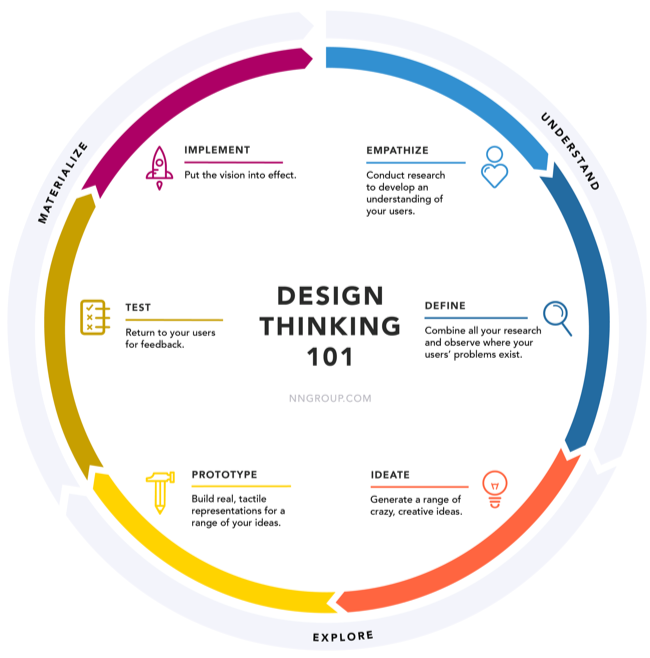
\includegraphics[width=0.85\textwidth]{res/design_thinking.png}
  \caption{Design Thinking 101 \citep[Quelle:][]{designthinking}}
  \label{fig:exintink}
\end{figure}
% label brauch man für verlinkungen, also in diesem fall unnötig
%\label{sec:refUeb1}

\section{EMPATHIZE}\label{EMPATHIZE}
\subsection{Beschreibung des Projektumfeldes}\label{Beschreibung des Projektumfeldes}
Beschreiben Sie unter diesem Punkt kurz das Umfeld (Ihr Unternehmen/ ihre Einrichtung/ Institution/ Verein) indem das Multimediaprodukt eingesetzt werden soll.
Welche Besonderheiten sind dort evtl. anzutreffen?
Gibt es Dinge, die man bei der Gestaltung eines Multimediaproduktes besonders beachten muss?

\subsection{Beschreibung der Zielgruppe}\label{Beschreibung der Zielgruppe}
Hier sollen Sie Ihre Zielgruppe beschreiben.
Welche Altersgruppe umfasst ihre Zielgruppe?
Liegen Einschränkungen vor?
Besondere Interessen oder Ansprüche?
Usw


\section{DEFINE}\label{DEFINE}


\subsection{Befragung von potentiellen Nutzern und/oder Kollegen}\label{Befragung von potentiellen Nutzern und/oder Kollegen}
Stellen Sie bitte folgende Fragen an Probanden Ihrer Zielgruppe/ oder falls diese nicht erreichbar sind Ihren Kollegen:

Fällt Ihnen spontan ein digitales Produkt/ Anwendung ein, die Sie ich im {Projektumfeld} wünschen würden?

Welche Abläufe/ Strukturen/ organisatorische Regelungen könnten in Ihrer Meinung nach (im Projektumfeld) verbessert werden?

Welche Ausgabemedien (Tablet, Smartphone, …) nutzen Sie am liebsten?

Kennen Sie eine digitale App/ Anwendung, die Sie sich gerne auch im Kontext {Ihres Projektumfeldes} vorstellen können?

(Gerne können Sie auch weitere Fragen formulieren, die Sie an die Probanden stellen und die Ihnen Inspirationen liefern können. )


\subsection{Ergebnisse der Befragung}\label{Ergebnisse der Befragung}
Stellen Sie hier bitte kurz die Ergebnisse der Befragung dar.

\subsection{Projektziel}\label{Projektziel}
Leiten Sie aus den Ergebnissen der Befragung ein Projektziel ab, welches Sie kurz formulieren

% Seitenumbruch
% \newpage

\section{IDEATE}\label{IDEATE}


\subsection{Produktidee (zur Lösung des Projektziels)}\label{Produktidee (zur Lösung des Projektziels) }
Entwickeln Sie eine Produktidee, diese Sie gerne als Prototyp als Lösungsansatz für das Projektziel umsetzen möchten.

\section{PROTOTYPE}\label{PROTOTYPE}

\subsection{Geplantes Ausgabemedium}\label{Geplantes Ausgabemedium}
Welches Ausgabemedium wollen Sie gerne für Ihren Prototypen nutzen? Mit kurzer Begründung bitte. Beachten Sie dazu bitte sowohl die Ergebnisse Ihrer Benutzerbefragung als auch die Voraussetzungen der Projektumgebung.

\subsection{Geplanter Medieneinsatz}\label{Geplanter Medieneinsatz}
Welche Medien (Audio/ Video/ Bild/ …) planen Sie einzusetzen?




% falls man lieber eine Datei pro Kapitel bevorzug, kann man dies auch einfach realisieren, indem man diese wie folgt einbindet
%\input{src/kapitel01.tex}
%\input{src/kapitel02.tex}
%\input{src/kapitel03.tex}
% diese müssen dann natürlcih in dem Ordner vorliegen


\newpage

% nocite lässt alle Werke anzeigen, auch solche die nicht verlinkt sind.
%\nocite{*}
\printbibliography[heading=bibintoc]

\newpage

% Abbildungsverzeichnis anzeigen
\listoffigures
\addcontentsline{toc}{section}{\listfigurename}

\newpage


%!TEX root = ../konzeptpapier.tex
% Erklaerung der Selbststaendigkeit.
% Footer wird in config.tex durch \AtEndDocument{\ofoot{}} angepasst
\section*{Erklärung der Selbständigkeit}
\addcontentsline{toc}{section}{Erklärung der Selbständigkeit}
Ich versichere, dass ich die vorliegende schriftliche Prüfungsleistung selbständig verfasst, keine anderen als die angegebenen Quellen und Hilfsmittel verwendet habe und die Stellen, die anderen Werken im Wortlaut oder dem Sinn nach entnommen sind, im Text jeweils mit Quellenbelegen kenntlich gemacht habe. Die Arbeit ist noch nicht anderweitig für Prüfungszwecke vorgelegt worden.
\\
\\
\\
\\
\\

\parbox{5cm}{\centering  \ortderarbeit, \today\hrule\strut\centering\footnotesize Ort, Datum}
\hfill
\vspace{-2cm}
\parbox{6cm}{\centering {\color{white} X} \hrule\strut \centering\footnotesize Unterschrift}
%\vspace{-2cm} %hochschieben
%\includegraphics[width=0.4\textwidth,heigth=12pt]{res/Unterschrift.png}
%\vspace{2cm} % wieder runter


\end{document}

